\begin{figure}[htbp]
\centering
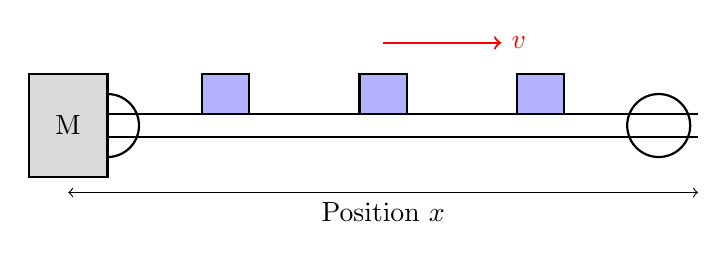
\begin{tikzpicture}
    % Belt
    \draw[thick] (0,0) -- (8,0);
    \draw[thick] (0,0.3) -- (8,0.3);

    % Rollers
    \draw[thick] (0.5,0.15) circle (0.4);
    \draw[thick] (7.5,0.15) circle (0.4);

    % Motor
    \draw[thick, fill=gray!30] (-0.5,-0.5) rectangle (0.5,0.8);
    \node at (0,0.15) {M};

    % Items on belt
    \foreach \x in {2,4,6} {
        \draw[thick, fill=blue!30] (\x-0.3,0.3) rectangle (\x+0.3,0.8);
    }

    % Speed
    \draw[->, thick, red] (4,1.2) -- (5.5,1.2) node[right] {$v$};

    % Position
    \draw[<->] (0,-0.7) -- (8,-0.7) node[midway, below] {Position $x$};
\end{tikzpicture}
\caption{Conveyor belt system with motor drive.}
\label{fig:conveyor}
\end{figure}
